\begin{chapter}{Estado de la tecnología}
    
    \lettrine{C}{on} el desarrollo de las tecnologías web y la comercialización por parte de grandes empresas de su infraestructura, los servicios \textit{Infrastructure as a Service} (IaaS) han ganado una popularidad considerable, con ello también se han desarrollado herramientas software dedicadas a la gestión de infraestructura para la implementación de sistemas Cloud Computing. Algunas de estas son VMware Cloud Foundation (creado en 2011), OpenStack (creado en 2010) o Apache CloudStack (creado en 2012). Estos productos proveen software que permite construir una infraestructura virtualizada sobre un conjunto de recursos físicos, con el objetivo de separar la administración de la capa física de la capa virtual para simplificar y automatizar la gestión y escalabilidad de los recursos. Proponen un modelo que persigue reducir costes de gestión de la infraestructura y aumentar la disponibilidad del servicio, es decir, aumentar la eficiencia de la infraestructura física.
    A lo largo de este capítulo se expone la solución Cloud propuesta para ser implementada en la infraestructura del CITIC indicando las razones de su elección y sus principales características.

\begin{section}{Servicio Cloud}    

    Como ya se ha visto, en el mercado existen varias alternativas que se pueden utilizar para cumplir los objetivos del proyecto. Finalmente, se ha escogido el producto \textbf{VMware Cloud Foundation} (VCF) ya que al ser del mismo proveedor, todos sus componentes se integra perfectamente con los componentes de VMware ya instalados en la infraestructura, por lo tanto, su mantenimiento es más sencillo y su funcionamiento más eficiente. También es posible integrar soluciones de otras compañías pero, al estar fuera del ecosistema de VMware podrían producirse problemas de compatibilidad entre versiones a largo plazo con los productos existentes en la infraestructura del CITIC. Utilizando los productos de un mismo proveedor se asegura el soporte del software instalado y la obtención del máximo rendimiento de cada componente.
        
    \begin{subsection}{VMware Cloud Foundation}
    
        Esta solución de VMware virtualiza todas las capas de la infraestructura combinando cuatro de sus productos. Utiliza \textbf{VMware vSphere} para virtualizar y gestionar el cómputo, \textbf{VMware vSAN} para virtualizar y gestionar el almacenamiento, \textbf{VMware NSX-T} para la virtualización y gestión de la red, y \textbf{VMware vRealize Suite} para gestionar las operaciones de la infraestructura virtual como el aprovisionamiento de recursos. Todos estos servicios juntos convierten el CPD en un Software Defined Datacenter (SDDC), un entorno donde existe una infraestructura física que se abstrae en una capa virtual para separar la gestión de ambas y poder modificar la infraestructura virtual según las necesidades de los usuarios sin necesidad de modificar la configuración de la infraestructura física, y que permite a los usuarios aprovisionar recursos, construyendo así un servicio de Cloud Computing. Con esta estructura se obtienen las siguientes características:
        
    \begin{itemize}
    
        \item Servicios software con integración nativa: ofrece un conjunto de servicios software para el almacenamiento, red, seguridad y gestión del servicio Cloud. Estos servicios se integran de forma nativa con la infraestructura minimizando las tareas de configuración y administración.
    
        \item Escalabilidad y elasticidad de los recursos: la capacidad de la infraestructura se puede modificar de forma sencilla gracias a la automatización del ciclo de vida de todos los elementos y al desacople entre las dos capas (la física y la virtual).
    
        \item Supervisión de los recursos: monitoriza los recursos con reconocimiento de aplicaciones y solución de problemas, permitiendo conocer todos los eventos que tienen lugar en la infraestructura. También permite establecer políticas de seguridad en cuanto al acceso a los recursos y la red.
    
        \item Aprovisionamiento automatizado: permite la obtención de recursos de forma automática incluyendo servicios de red, almacenamiento y cómputo. Los componentes de la infraestructura virtualizada se encargan de la reserva de los recursos y de todas las operaciones necesarias para llevarla acabo.
    
        \item Ciclo de vida automatizado: automatiza las operaciones de gestión previas, iniciales y posteriores de la plataforma para simplificar y coordinar su gestión. En estas tareas incluye el despliegue de la plataforma y su implementación, la escalabilidad de los recursos físicos y la instalación de actualizaciones para cada componente software.
    
    \end{itemize}
    \begin{figure}[h!]
        \centering
        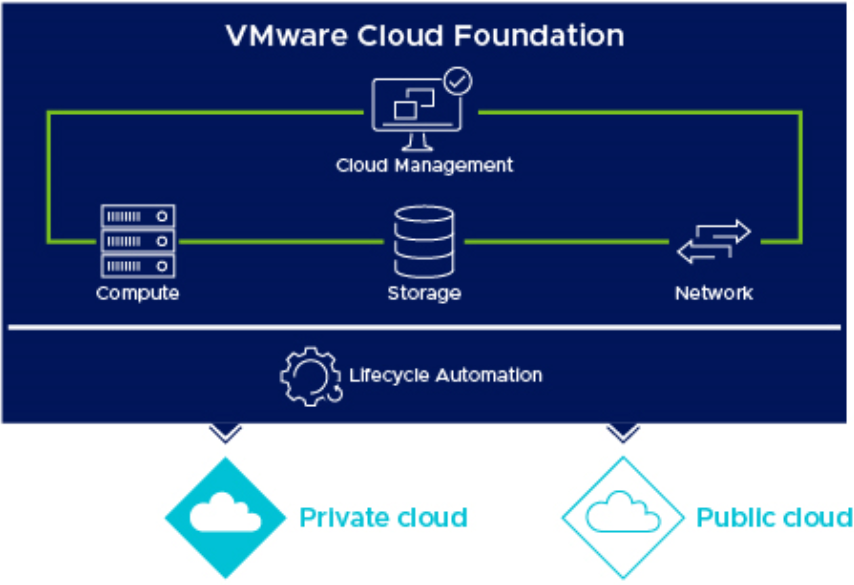
\includegraphics[width=0.6\textwidth]{imaxes/cap2recursos/overviewCF.png}
                \caption{Estructura de VMare Cloud Foundation.}
        \label{fig:Cloud-Foundation-Overview}
        \end{figure}
        \FloatBarrier
        \begin{figure}[h]
            \centering
            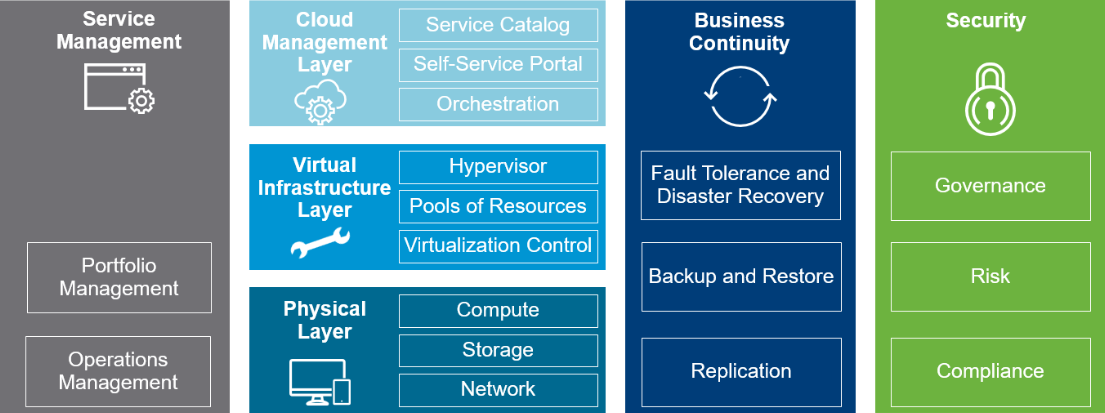
\includegraphics[width=0.8\textwidth]{imaxes/cap2recursos/SDDCoverview.png}
            \caption{Elementos de un SDDC gestionado con VMware Cloud Foundation.}
            \label{fig:layers-Sddc}
        \end{figure}
        \FloatBarrier
    \end{subsection}
    
    \begin{subsection}{Componentes de VMware Cloud Foundation}
    \label{subsubsect:cfcomponents}
    
    Ya se ha visto que VCF está formado por cuatro productos principales. En este apartado se describirán las características de esos cuatro componentes más el servicio que los coordina\footnote{Las características del componente VMware vSphere son las mismas que las descritas en el punto \ref*{subsec:softwareinstalado}}. Se utilizará la versión 4.0 de VMware Cloud Foundation lo cual implica que se implementarán las versiones\cite{componentesCloudFound} 4.0 de SDDC Manager, 7.0.0 de VMware vSphere, 7.0.0 de VMware vSAN, 3.0 de VMware NSX-T y 8.1 de VMware vRealize Suite.
    \begin{figure}[h]
        \centering
            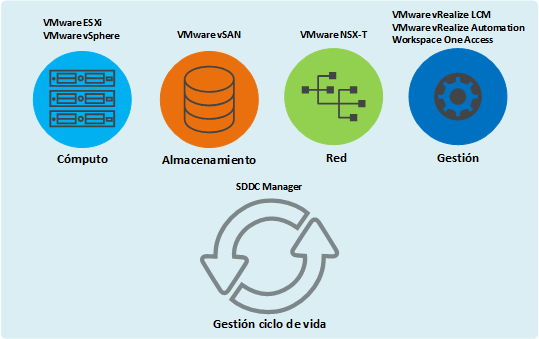
\includegraphics[width=0.6\textwidth]{imaxes/VCF-componentes/ComponentesVCF.png}
            \caption{Partes de un SDDC y componentes de VCF que las implementan.}
            \label{fig:componentes-funciones-VCF}
        \end{figure}
        \FloatBarrier
    \begin{subsubsection}{SDDC Manager}
        SDDC Manager se encarga de gestionar el ciclo de vida de todos los componentes de VCF, esto incluye el despliegue de cada uno, su configuración y la obtención e instalación de actualizaciones. Centraliza la gestión de las licencias y certificados de cada componente y administra el aprovisionamiento de nuevos recursos físicos para el SDDC y los ya existentes.
    \end{subsubsection}
    
    \begin{subsubsection}{VMware vSAN}
        VMware vSAN virtualiza el almacenamiento del SDDC. Permite gestionar de forma centralizada, desde la interfaz de vSphere Web Client, el sistema de almacenamiento sin necesidad de tener que modificar la configuración física. El sistema de almacenamiento se abstrae para formar único datastore sobre el que se establecen políticas de uso y disponibilidad. El acceso por parte de cada host al datastore se realiza con el protocolo IP, a través de una subred dedicada al servicio. Con VMware vSAN, el datastore está formado por discos de almacenamiento que se organizan en grupos que se asignan a un host. Los grupos pueden tener configuración \textit{Hybrid}, que combina discos HDD y SDD, o configuración \textit{All-Flash} que solo utiliza SSD y por lo tanto tiene mayor rendimiento. Dentro de cada grupo existe un disco de caché y al menos un disco de capacidad donde se almacenan los datos persistentes\cite{operacionesVSAN}. 
        % En el modo \textit{All-Flash}\footnote{Solo se describe el modo \textit{All-Flash} porque es la configuración recomendada por VMware.} la operación de lectura se realiza directamente sobre los discos de capacidad y la operación de escritura se hace sobre el disco caché que posteriormente escribe los datos en el disco de capacidad.
        
        \begin{figure}[h]
        \centering
            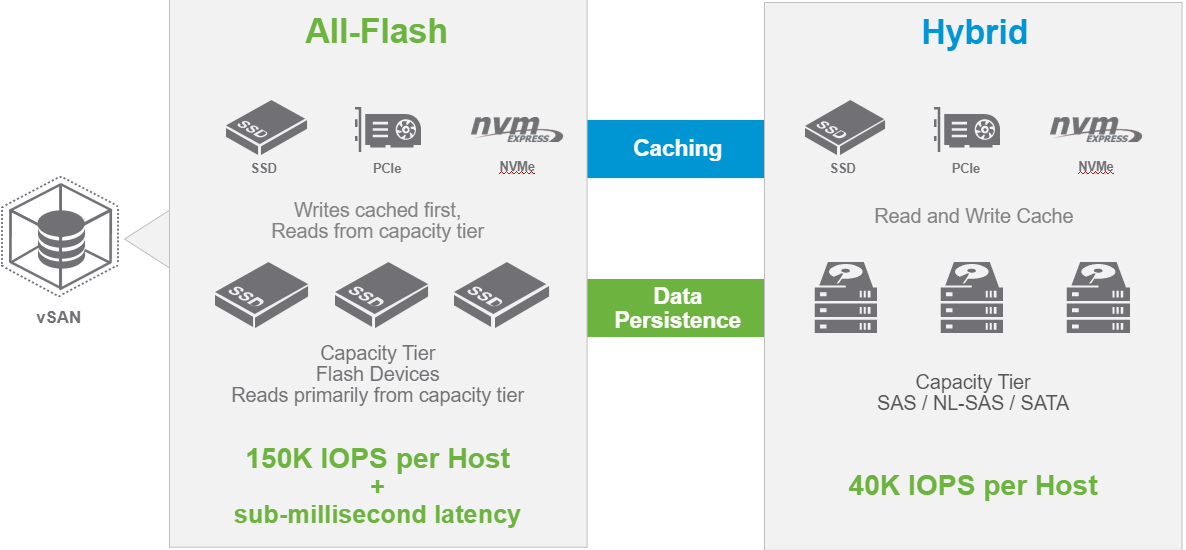
\includegraphics[width=0.6\textwidth]{imaxes/cap2recursos/rendimientoVSAN.png}
            \caption{Configuración \textit{All-Flash} y configuración \textit{Hybrid} en vSAN}
            \label{fig:performance-Hybrid-AllFlash-vSAN}
        \end{figure}
        \FloatBarrier
    \end{subsubsection}
    
    \begin{subsubsection}{VMware NSX-T}
        VMware NSX-T virtualiza la red del SDDC. Abstrae los componentes físicos de la red para generar una red virtual desacoplada de la infraestructura física, esta se configura sin modificar la red física y para ello aporta servicios de red virtualizados y la posibilidad de crear y extender subredes sobre la infraestructura. Internamente tiene tres componentes, NSX-T Manager, NSX-T Controller y NSX-T Edge. El primero, es el punto de acceso a la configuración de VMware NSX-T y el que almacena y transmite la configuración establecida, el segundo controla las redes y se encarga de informar sobre el estado y la configuración de las redes virtuales. El último componente, NSX-T Edge, proporciona servicios de red y enrutamiento a las redes virtuales. Los hosts que están integrados en VMware NSX-T se encargan de controlar el tráfico y monitorizar las conexiones que mantiene VMware NSX-T.
        % El control del tráfico y la monitorización de las conexiones se hace desde el componente \textbf{Transport Node} (TN) con la información que recibe de las instancias de NSX-T Controller. Existen dos tipos de TNs, \textbf{Hypervisor Transport Node} que son hosts con ESXi instalado y que están configurados para correr los servicios de VMware NSX-T, y \textbf{NSX-T Edge Node} que se trata de una \textit{appliance} instalada en una VM o sobre un host físico para proveer un conjunto de servicios de red centralizados para las redes virtuales de VMware NSX-T.
        \begin{figure}[h!]
            \centering
                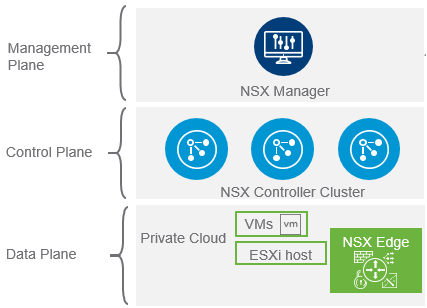
\includegraphics[width=0.6\textwidth]{imaxes/VCF-componentes/nsx-t-layers.png}
                \caption{Componentes de VMware NSX-T y capas en las que se dividen}
                \label{fig:nsx-t-components}
            \end{figure}
            \FloatBarrier
    \end{subsubsection}
    
    \begin{subsubsection}{VMware vRealize Suite}
        VMware vRealize Suite agrupa un conjunto de productos que si bien no son obligatorios para desplegar VCF, aportan funcionalidades extra que completan la formación del SDDC y del servicio Cloud. Los productos que se utilizarán en este proyecto son \textbf{vRealize Suite Lifecycle Manager} dedicado a gestionar el despliegue, actualizaciones, certificados y licencias de los productos que forman VMware vRealize, \textbf{Workspace One Access} dedicado a gestionar los usuarios y ser el punto de acceso centralizado de las aplicaciones de VMware vRealize Suite y, finalmente, \textbf{vRealize Automation} el cual permite a los usuarios del SDDC diseñar y aprovisionar un conjunto de recursos de la infraestructura según sus necesidades y de forma automatizada mientras el administrador puede limitar la cantidad de recursos que se consumen.
    \end{subsubsection}
    \end{subsection}
    
    \begin{subsection}{Costes de implementación}
        Los principales costes a la hora de implementar VMware Cloud Foundation en la infraestructura de producción del CITIC son aquellos relacionados con la adquisición de licencias y soporte de los productos. Cada componente de VMware Cloud Foundation requiere su propia licencia\cite{licenses}. El precio de cada licencia dependerá del número de CPUs físicas sobre las que se va usar esta plataforma por lo que, como en la infraestructura hay un total de ocho hosts con dos CPUs cada uno, \underline{el precio por cada componente} es el siguiente:
        \begin{itemize}
            \item \textbf{SDDC Manager}: 18.000€\footnote{Para la edición \textit{Advanced} de VMware Cloud Foundation.} por CPU y 6.500€ anuales de soporte por cada CPU. El precio total de la licencia es de 288.000€ y 104.000€ anuales de soporte por 16 CPUs.
            \item \textbf{VMware vSphere}: 4.000€\footnote{Para la edición \textit{Standard} de VMware vSphere.} por CPU. El precio total de la licencia es de 64.000€ por 16 CPUs y el precio anual por las tareas de soporte es de 16.000€.
            \item \textbf{VMware vCenter}: 6.000€\footnote{Para la edición \textit{Standard} de VMware vCenter} por una licencia que permite usar VMware vCenter sobre todos los hosts del entorno. El precio anual por las tareas de soporte es de 1.500€.
            \item \textbf{VMware vSAN}: 4.000€\footnote{Para la edición \textit{Advanced} de VMware vSAN.} por CPU. El precio total de la licencia es de 64.000€ por 16 CPUs y el precio anual por las tareas de soporte es de 16.000€.
            \item \textbf{VMware NSX-T}: 5.300€\footnote{Para la edición \textit{Advanced} de NSX.} por CPU. El precio total de la licencia es de 84.400€ por 16 CPUs y el precio anual por las tareas de soporte es de 21.100€.
            \item \textbf{VMware vRealize Suite 2019}: 1.500€ por CPU. El precio total de la licencia es de 24.000€ por 16 CPUs y el precio anual por las tareas de soporte es de 6.000€.
        \end{itemize}
        El precio total de todas las licencias necesarias para el entorno, teniendo en cuenta que hay 16 CPUs, sería igual a 530.400€, y el precio total por las tareas de soporte sería igual a 164.600€ anuales. En caso de que ya estén instalados algunos de los componentes entonces solo se requieren licencias para aquellos componentes que aún no están en el entorno. En el caso del entorno inicial, los componentes que ya están instalados son VMware vSphere, VMware vCenter Server. Esto hace que el \underline{coste real para implementar VMware Cloud Foundation} en el entorno sea igual a 460.400€, ya que solo son necesarias licencias para los componentes SDDC Manager, VMware vSAN, VMware NSX-T y VMware vRealize Suite 2019. El coste total de la instalación y mantenimiento de la plataforma VMware Cloud Foundation sobre la infraestructura del CITIC es el siguiente:
        \begin{itemize}
            \item \textbf{Licencias}: 460.400€ en total.
            \item \textbf{Soporte}: 164.600€ anuales.
        \end{itemize}
    \end{subsection}
    
    \end{section}
\end{chapter}